\quad Al igual que en el an\'alisis previo, realizamos mediciones de los estimadores variando el par\'ametro de entrada sobre las mismas poblaciones mencionadas.\\

\quad El par\'ametro que se var\'ia en todos los estimadores representa la cantidad de \textit{buckets}, aunque en el estimador de pasos distribuidos se lo llaman \textit{steps}.

\subsubsection{Distribuci\'on uniforme}

\begin{itemize}
\item \textbf{Operaci\'on por igualdad} \\

\quad lala\\

\begin{figure}[H]
	  \begin{center}
	    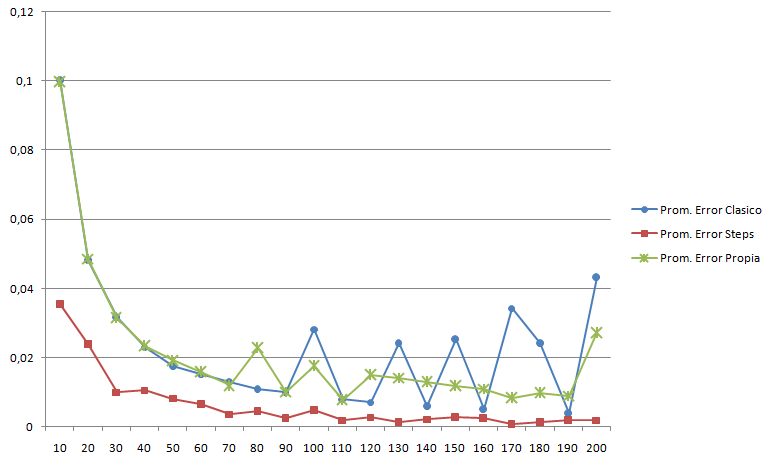
\includegraphics[scale=.80]{imagenes/parametroVariableC0Eq.png}
	    \caption{Error promedio de la Columna C0 de la tabla brindada por la materia} 
	    \label{fig:C2_variando_valor}
	  \end{center}
\end{figure}

\quad lala \\

\item \textbf{Operaci\'on por mayor} \\

\quad lala \\

\begin{figure}[H]
	  \begin{center}
	    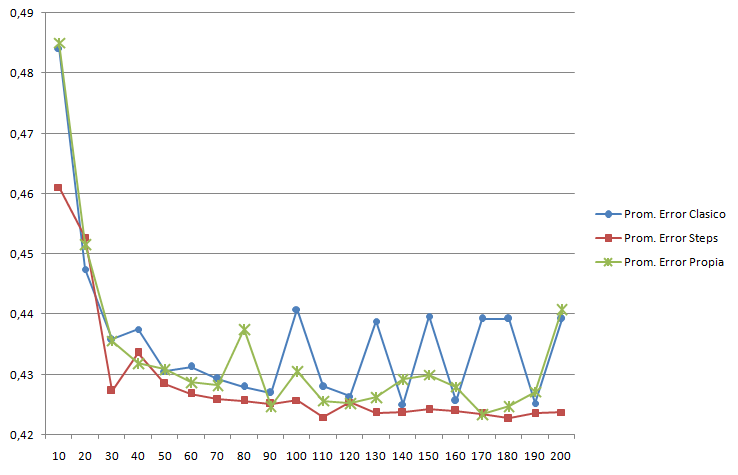
\includegraphics[scale=.80]{imagenes/parametroVariableC0Greater.png}
	    \caption{Error promedio de la Columna C0 de la tabla brindada por la materia} 
	    \label{fig:C2_variando_valor}
	  \end{center}
\end{figure}

\quad lala \\

\end{itemize}

\subsubsection{Distribuci\'on normal}

\begin{itemize}
\item \textbf{Operaci\'on por igualdad} \\

\quad lala \\

\begin{figure}[H]
	  \begin{center}
	    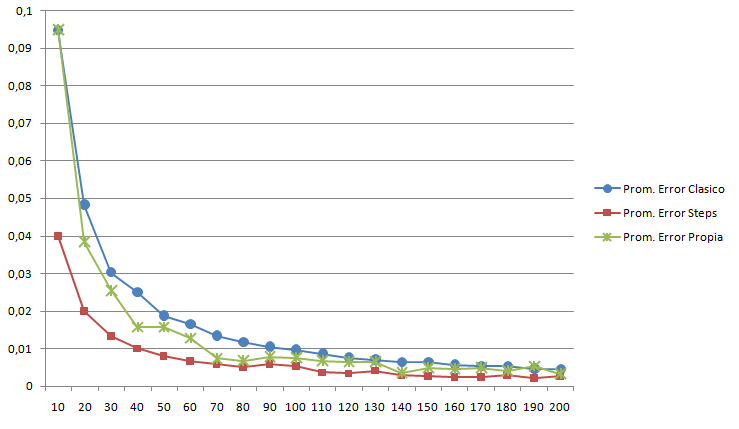
\includegraphics[scale=.80]{imagenes/parametroVariableC2Eq.png}
	    \caption{Error promedio de la Columna C2 de la tabla brindada por la materia} 
	    \label{fig:C2_variando_valor}
	  \end{center}
\end{figure}

\quad lala \\

\item \textbf{Operaci\'on por mayor} \\

\quad lala \\

\begin{figure}[H]
	  \begin{center}
	    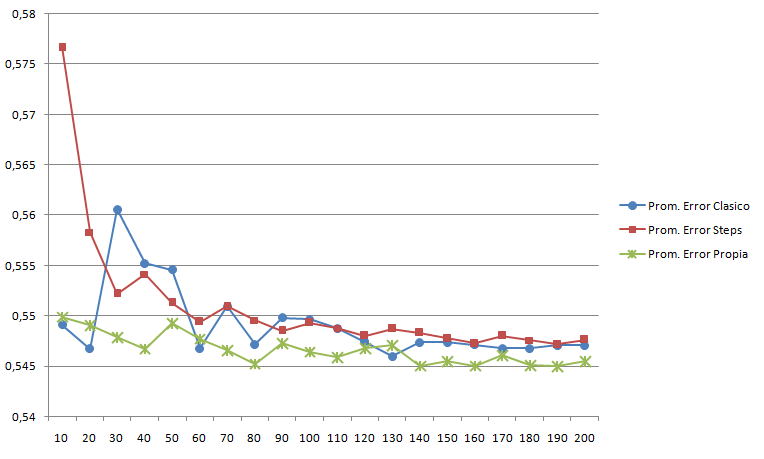
\includegraphics[scale=.80]{imagenes/parametroVariableC2Greater.png}
	    \caption{Error promedio de la Columna C2 de la tabla brindada por la materia} 
	    \label{fig:C2_variando_valor}
	  \end{center}
\end{figure}

\quad lala \\

\end{itemize}